%% LyX 2.3.7 created this file.  For more info, see http://www.lyx.org/.
%% Do not edit unless you really know what you are doing.
\documentclass[english]{beamer}
\usepackage{amsbsy}
\usepackage{amstext}
\usepackage{amssymb}
\usepackage{fontspec}
\usepackage{calc}
\usepackage{graphicx}
\PassOptionsToPackage{normalem}{ulem}
\usepackage{ulem}
\ifx\hypersetup\undefined
  \AtBeginDocument{%
    \hypersetup{unicode=true,
 bookmarks=true,bookmarksnumbered=true,bookmarksopen=true,bookmarksopenlevel=1,
 breaklinks=true,pdfborder={0 0 0},pdfborderstyle={},backref=section,colorlinks=true,pdftitle={线性代数复习(一)},
 pdfauthor={gwzhang},
 pdfsubject={数学}}
  }
\else
  \hypersetup{unicode=true,
 bookmarks=true,bookmarksnumbered=true,bookmarksopen=true,bookmarksopenlevel=1,
 breaklinks=true,pdfborder={0 0 0},pdfborderstyle={},backref=section,colorlinks=true,pdftitle={线性代数复习(一)},
 pdfauthor={gwzhang},
 pdfsubject={数学}}
\fi

\makeatletter

%%%%%%%%%%%%%%%%%%%%%%%%%%%%%% LyX specific LaTeX commands.
\XeTeXdashbreakstate 0
%% Because html converters don't know tabularnewline
\providecommand{\tabularnewline}{\\}

%%%%%%%%%%%%%%%%%%%%%%%%%%%%%% Textclass specific LaTeX commands.
% this default might be overridden by plain title style
\newcommand\makebeamertitle{\frame{\maketitle}}%
% (ERT) argument for the TOC
\AtBeginDocument{%
  \let\origtableofcontents=\tableofcontents
  \def\tableofcontents{\@ifnextchar[{\origtableofcontents}{\gobbletableofcontents}}
  \def\gobbletableofcontents#1{\origtableofcontents}
}

%%%%%%%%%%%%%%%%%%%%%%%%%%%%%% User specified LaTeX commands.
\usetheme{Singapore}
\usefonttheme[onlymath]{serif}
% or ...
\usepackage{ctex}
\setbeamercovered{transparent}
% or whatever (possibly just delete it)

\makeatother

\usepackage{polyglossia}
\setdefaultlanguage[variant=american]{english}
\begin{document}
\title{线性代数复习(一) 解线性方程组}
\institute{a freshman at CUG Computer Science}
\author{AUGPath}

\makebeamertitle
\global\long\def\R{\mathbb{R}}%

\begin{frame}{导引: 摘自Linear Algrbra and its Applications}

This course is potentially the most interesting and worthwhile undergraduate
mathematics course you will complete. In fact, some students have
written or spoken to us after graduation and said that they still
use this text occasionally as a reference in their careers at major
corporations and engineering graduate schools. The following remarks
offer some practical advice and information to help you master the
material and enjoy the course.

...

In a practical sense, linear algebra is a language. You must learn
this language the same way you would a foreign language—with daily
work. Material presented in one section is not easily understood unless
you have thoroughly studied the text and worked the exercises for
the preceding sections. Keeping up with the course will save you lots
of time and distress!
\end{frame}
%
\begin{frame}{概览: 两条线索}

对于$\begin{cases}
a_{11}x_{1}+a_{12}x_{2}+\cdots+a_{1n}x_{n} & =b_{1}\\
\cdots\\
a_{m1}x_{1}+a_{m2}x_{2}+\cdots+a_{mn}x_{n} & =b_{m}
\end{cases}$的方程组我们应该怎样处理?
\begin{itemize}
\item 通过$n=1,n=2,\cdots,n=m$的时候去枚举未知数相等情形
\item 直接通过当前的情形去消元
\end{itemize}
\end{frame}
%

\section{第一条路线}
\begin{frame}{考虑小的情形}
\begin{itemize}
\item 解答: $\begin{cases}
a_{11}x_{1}+a_{12}x_{2} & =b_{1}\\
a_{21}x_{1}+a_{22}x_{2} & =b_{2}
\end{cases}$
\item 解答: $\begin{cases}
a_{11}x_{1}+a_{12}x_{2}+a_{13}x_{3} & =b_{1}\\
a_{21}x_{1}+a_{22}x_{2}+a_{23}x_{3} & =b_{2}\\
a_{31}x_{1}+a_{32}x_{2}+a_{33}x_{3} & =b_{3}
\end{cases}$.
\begin{itemize}
\item 小技巧: 可以借助上面的问题, 先把某些内容看做常数. 
\item 提示: 试图引入记号$ad-bc=\begin{vmatrix}a & b\\
c & d
\end{vmatrix}$.
\end{itemize}
\item 一般的规律: 一个很好玩的递推关系:
\[
D_{i}=\sum_{i=1}^{n}(-1)^{1+i}a_{1i}M_{1i}.
\]
 
\end{itemize}
\end{frame}
%
\begin{frame}{展开说说?}
\begin{itemize}
\item 递推关系式太讨厌! 
\item 用工具试一试. (见\textcolor{teal}{\uwave{det.py}})
\item 发现了什么?
\end{itemize}
\end{frame}
%
\begin{frame}{跑题: 时间复杂度}

Q: 小于2095728218的正质数有几个?
\begin{itemize}
\item 于是产生了各种各样的代码.
\begin{itemize}
\item ``我跑了好久, 可是电脑不给我答案啊!''
\item 计算机1s大约能运行1e8$\sim$1e9次运算(可以粗略的认为走过一次简单的一行算一次运算)
\end{itemize}
\end{itemize}
那么刚刚的程序时间复杂度是多少? 
\begin{itemize}
\item 少说定义, 实际跑一下看看
\item 这么多东西, 谁看得懂?
\end{itemize}
\end{frame}
%
\begin{frame}{跑题: 工具的力量}
\begin{itemize}
\item 正常人谁都看不懂, 但是工具可以啊
\item 学校开的Python课程感觉落不到实处, 但是现在就是机会
\item 高考的时候如果让带电脑, 那不有手就行? (针对2022年及以前的卷子)
\begin{itemize}
\item Wolfram Alpha, Wolfram Mathematica, MATLAB, 再也不用担心计算错误了
\item 圆锥曲线的联立的那种级别的计算, $\sim1\text{s}$就能出答案
\item 导数题估计精确度至少是$1\times10^{-5}$的级别
\end{itemize}
\item Python包: sympy(符号计算)
\begin{itemize}
\item 有了玩耍的基础
\end{itemize}
\end{itemize}
\end{frame}
%
\begin{frame}{!发现了什么?}

\begin{tabular}{|c|c|c|c|}
\hline 
$(i_{1},i_{2},i_{3})$ & $a_{1i_{1}},a_{2i_{2}},a_{3i_{3}}$的符号 & 换序方法 & 换序次数\tabularnewline
\hline 
\hline 
(1,2,3) & + & / & 0\tabularnewline
\hline 
(2,3,1) & + & $1\leftrightarrow3,1\leftrightarrow2$ & 2\tabularnewline
\hline 
(3,1,2) & + & $1\leftrightarrow3,2\leftrightarrow3$ & 2\tabularnewline
\hline 
(1,3,2) & - & $2\leftrightarrow3$ & 1\tabularnewline
\hline 
(2,1,3) & - & $1\leftrightarrow2$ & 1\tabularnewline
\hline 
(3,2,1) & - & $1\leftrightarrow2,2\leftrightarrow3,1\leftrightarrow3$ & 3\tabularnewline
\hline 
\end{tabular}

猜测: 
\[
|A|=\sum_{(i_{1},\cdots.i_{n})}(-1)^{\tau(i_{1},\cdots.i_{n})}a_{1i_{1}}a_{2i_{2}}\cdots a_{ni_{n}}.
\]
\begin{itemize}
\item 可以使用数学归纳法证明. 
\end{itemize}
\end{frame}
%
\begin{frame}{!逆序数(inversion number)}
 
\begin{itemize}
\item Def. 排列(permutation)
\item Def. 逆序数, 奇(odd)排列, 偶(even)排列.
\item Def. 对换(swap).
\item Th. 排列中任意两个元素对换, 排列改变奇偶性.
\end{itemize}
\end{frame}
%
\begin{frame}{什么样的行列式是好算的?}
\begin{itemize}
\item 全是0. (Trivial case)
\item 对角线上全是0. 
\item 上/下三角.
\item 一般的$\stackrel{\text{转\text{换}}}{\longrightarrow}$特殊的
\item 这个思想在后面学习对角化与特征值、二次型与标准形也会遇见. 
\end{itemize}
\end{frame}
%
\begin{frame}{!行列式的性质}

\[
|A|=\sum_{(i_{1},\cdots.i_{n})}(-1)^{\tau(i_{1},\cdots.i_{n})}a_{1i_{1}}a_{2i_{2}}\cdots a_{ni_{n}}.
\]
\begin{itemize}
\item 转置
\item 互换
\item 线性性
\end{itemize}
\end{frame}
%
\begin{frame}{例子: 基本概念. 多项式与行列式}
\begin{enumerate}
\item $\begin{vmatrix}11 & 45 & 14\\
19 & 19 & 81\\
0 & 11 & 45
\end{vmatrix}=-35945.$
\item $D=\begin{vmatrix}a_{1}+x & a_{2} & a_{3} & a_{4}\\
-x & x\\
 & -x & x\\
 &  & -x & x
\end{vmatrix}=x^{3}\left(x+\sum_{i=1}^{4}a_{i}\right).$
\item $\begin{vmatrix}x & 0 & 0 & \cdots & 0 & a_{0}\\
-1 & x & 0 & \cdots & 0 & a_{1}\\
0 & -1 & x & \cdots & 0 & a_{2}\\
 &  & \vdots & \ddots & \vdots & \vdots\\
0 & 0 & 0 & \cdots & x & a_{n-2}\\
0 & 0 & 0 & \cdots & -1 & x+a_{n-1}
\end{vmatrix}=x^{n}+a_{n-1}x^{n-1}+\cdots+a_{0}.$
\end{enumerate}
\end{frame}
%
\begin{frame}{例子: 多项式与行列式, 分块行列式}
\begin{enumerate}
\item $\begin{vmatrix}x & 0 & 0 & \cdots & 0 & a_{0}\\
-1 & x & 0 & \cdots & 0 & a_{1}\\
0 & -1 & x & \cdots & 0 & a_{2}\\
 &  & \vdots & \ddots & \vdots & \vdots\\
0 & 0 & 0 & \cdots & x & a_{n-1}\\
0 & 0 & 0 & \cdots & -1 & a_{n}
\end{vmatrix}=\sum_{i=0}^{n}a_{i}x^{i}.$
\item $D=\begin{vmatrix}\mathbf{A}_{n\times n} & \mathbf{0}\\
\mathbf{C} & \mathbf{B}_{m\times m}
\end{vmatrix}=\mathbf{A}_{n\times n}\mathbf{B}_{m\times m}$
\end{enumerate}
\end{frame}
%
\begin{frame}{!展开的智慧: 关于代数余子式}
\begin{itemize}
\item 能不能不总是第一列(行)开始展开? 
\begin{itemize}
\item 能不能同时选择多行展开?
\item 
\[
D_{i}=\sum_{i=1}^{n}(-1)^{1+i}a_{1i}M_{1i}=\sum_{i=1}^{n}a_{1i}A_{1i}
\]
\item Def. 余子式, 代数(带着符号的)余子式.
\item Prop. 
\[
\sum_{k=1}^{n}a_{ki}A_{kj}=D\delta_{ij};\sum_{k=1}^{n}a_{ik}A_{jk}=D\delta_{ij}.
\]
\end{itemize}
\item 代数余子式有``操纵行列式''的感觉.
\end{itemize}
\end{frame}
%
\begin{frame}{例子: 操纵行列式}

设4阶行列式$D_{4}=\begin{vmatrix}a & b & c & d\\
c & b & d & a\\
d & b & c & a\\
a & b & d & c
\end{vmatrix}$, 求$A_{14}+A_{24}+A_{34}+A_{44}$. 
\end{frame}
%
\begin{frame}{!多行展开行不行? Laplace定理}
\begin{itemize}
\item 选定行(列), 之后抽取所有可能的不重复的列(行), 赋予符号, 相加.
\item 就容易得到了
\[
D=\begin{vmatrix}\mathbf{A}_{n\times n} & \mathbf{0}\\
\mathbf{C} & \mathbf{B}_{m\times m}
\end{vmatrix}=\mathbf{A}_{n\times n}\mathbf{B}_{m\times m}
\]
\item 原始的方法其实有很好的启发: 矩阵的乘法. 
\item 行列式的乘积公式:
\[
\begin{vmatrix}a_{11}.. & a_{1n}\\
a_{n1}.. & a_{nn}
\end{vmatrix}\times\begin{vmatrix}b_{11}.. & b_{1n}\\
b_{n1}.. & b_{nn}
\end{vmatrix}=\begin{vmatrix}c_{11}.. & c_{1n}\\
c_{n1}.. & c_{nn}
\end{vmatrix}
\]
其中$c_{ij}=\sum_{i=1}^{n}a_{ik}b_{kj}.$
\end{itemize}
\end{frame}
%
\begin{frame}{证明Cramer法则}
\begin{itemize}
\item 引入$\delta_{ij}=\begin{cases}
1 & i=j\\
0 & i\neq j
\end{cases},$类似中国剩余定理的思想.
\item 其次线性方程组的行列式不等于0$\implies$只有0解. 
\item 由此就有了...
\item Thm1. 如果线性方程组系数的行列式$D\neq0$, 有唯一解.
\item Thm2. 如果\textbf{齐次}线性方程组的系数行列式$D\neq0$, 只有零解. 
\item 麻烦之处: 系数矩阵等于0会怎样?不是方阵?
\item 后续: 会用``秩''刻画相关的内容. 
\item 比较繁琐
\end{itemize}
\end{frame}

\section{第二条路线}

\begin{frame}{古人的智慧}

\noindent\fbox{\begin{minipage}[t]{1\columnwidth - 2\fboxsep - 2\fboxrule}%
今有上禾三秉,中禾二秉,下禾一秉,實三十九斗;上禾二秉,中禾三秉,下禾一秉,實三十四斗;上禾一秉,中禾二秉,下禾三秉,實二十六斗。問上、中、下禾實一秉各幾何? 

方程術曰,置上禾三秉,中禾二秉,下禾一秉,實三十九斗,於右方。中、左禾列如右方。以右行上禾遍乘中行而以直除。又乘其次,亦以直除。然以中行中禾不盡者遍乘左行而以直除。左方下禾不盡者,上為法,下為實。實即下禾之實。求中禾,以法乘中行下實,而除下禾之實。餘如中禾秉數而一,即中禾之實。求上禾亦以法乘右行下實,而除下禾、中禾之實。餘如上禾秉數而一,即上禾之實。實皆如法,各得一斗。–《九章算術》

https://ctext.org/library.pl?if=gb\&file=58466\&page=43%
\end{minipage}}

消元法: 
\begin{itemize}
\item 互换两个方程的位置
\item 某一个方程乘上$k$倍
\item 一个方程乘上$k$倍加到另一个上面去
\end{itemize}
\end{frame}
%
\begin{frame}{怎么表示?}
\begin{itemize}
\item 上述的三种情形是变量代换的特殊情况. 
\item 变量代换: $\begin{cases}
a_{11}x_{1}+a_{12}x_{2} & =c_{1}\\
a_{21}x_{1}+a_{22}x_{2} & =c_{2}
\end{cases}$与 $\begin{cases}
b_{11}y_{1}+b_{12}y_{2} & =x_{1}\\
b_{21}y_{1}+b_{22}y_{2} & =x_{2}
\end{cases}$ 
\item 得到$\begin{cases}
(a_{11}b_{11}+a_{12}b_{21})y_{1}+(a_{11}b_{12}+a_{12}b_{22})y_{2} & =c_{1}\\
(a_{21}b_{11}+a_{22}b_{21})y_{1}+(a_{21}b_{12}+a_{22}b_{22})y_{2} & =c_{2}
\end{cases}$, 系数矩阵是$\begin{pmatrix}a_{11}b_{11}+a_{12}b_{21} & a_{11}b_{12}+a_{12}b_{22}\\
a_{21}b_{11}+a_{22}b_{21} & a_{21}b_{12}+a_{22}b_{22}
\end{pmatrix}$
\item 
\[
\begin{pmatrix} &  &  & b_{11} & b_{12}\\
 &  &  & b_{21} & b_{22}\\
 &  &  & \downarrow & \downarrow\\
a_{11} & a_{12} & \rightarrow & a_{11}b_{11}+a_{12}b_{21} & a_{11}b_{12}+a_{12}b_{22}\\
a_{21} & a_{22} & \rightarrow & a_{21}b_{11}+a_{22}b_{21} & a_{21}b_{12}+a_{22}b_{22}
\end{pmatrix}
\]
\end{itemize}
\end{frame}
%
\begin{frame}{可以对线性方程组的系数进行表示}
\begin{itemize}
\item $\begin{cases}
a_{11}x_{1}+a_{12}x_{2}+\cdots+a_{1n}x_{n}=b_{1}\\
a_{21}x_{1}+a_{22}x_{2}+\cdots+a_{2n}x_{n}=b_{2}\\
\ \ \ \ \ \vdots\\
a_{m1}x_{1}+a_{m2}x_{2}+\cdots+a_{mn}x_{n}=b_{m}
\end{cases}$
\item $\begin{pmatrix}a_{11} &  & \cdots &  & a_{1n}\\
\\
\vdots &  & \ddots &  & \vdots\\
\\
a_{m1} &  & \cdots &  & a_{mn}
\end{pmatrix}$
\end{itemize}
\end{frame}
%
\begin{frame}{行列式为零或方程与未知量不一样多怎么办?}
\begin{itemize}
\item 代数学处理问题的方式一般是整体考虑
\item 而在代数层面上, 集合的整体性质是通过其中的运算关系来展示的, 所以我们需要研究矩阵集合上的运算.
\end{itemize}
\end{frame}
%
\begin{frame}{!矩阵及其运算}
\begin{itemize}
\item 转换的观念
\begin{itemize}
\item 地图 $\rightarrow$ 表
\item 方程 $\rightarrow$ 系数构成的表
\item 坐标系
\end{itemize}
\item Def. 矩阵(matrix), 行(row), 列(column), 元素(element). 
\item Def. 方阵(square), 行(列)矩阵, 对角阵, 零矩阵, 单位阵$\boldsymbol{E}$(有些课本$I_{n}$)
\end{itemize}
\end{frame}
%
\begin{frame}{案例: 电脑是如何对图形变换的}
\begin{itemize}
\item (以二维平面为例) 参看程序\textcolor{teal}{\uwave{transform.py}}.
\end{itemize}
\end{frame}
%
\begin{frame}{!矩阵的运算: 加法和数乘}
\begin{itemize}
\item 希望它是封闭的. 需要全体矩阵为$M$, 全体数字为$F$
\begin{itemize}
\item 这个``全体数字''的集合也要是封闭的
\end{itemize}
\item 运算规律: 交换律, 结合律
\end{itemize}
\end{frame}
%
\begin{frame}{!矩阵的运算: 与矩阵相乘}
\begin{itemize}
\item 回到了我们一开始的变量代换的视角.
\item 不满足交换律$\implies$左边乘, 右边乘
\item 有结合律$\implies$可以定义幂次方
\item 不满足交换律$\neq$所有矩阵都不可以交换. 如
\[
AE=EA;\qquad AB=E\iff BA=E
\]
\end{itemize}
\end{frame}
%
\begin{frame}{有趣的问题: 什么样的矩阵是可交换的?}

\href{https://en.wikipedia.org/wiki/Commuting_matrices}{可交换矩阵-维基百科}(commuting
matrices):
\begin{itemize}
\item Two diagonalizable matrices $A$ and $B$ commute ($AB=BA$) if they
are simultaneously diagonalizable (that is, there exists an invertible
matrix $P$ such that both ${\displaystyle P^{-1}AP}$ and ${\displaystyle P^{-1}BP}$
are diagonal). Converse is valid, provided that one of the matrices
has no multiple eigenvalues.
\item If A and B commute, they have a common eigenvector. If A has distinct
eigenvalues, and A and B commute, then A's eigenvectors are B's eigenvectors.
\item The property of two matrices commuting is not transitive.
\item ...
\end{itemize}
\end{frame}
%
\begin{frame}{!与行列式的关系: 矩阵数乘与取行列式}
\begin{itemize}
\item $k\begin{pmatrix}* & * & *\\
* & * & *\\
* & * & *
\end{pmatrix}=\begin{pmatrix}k* & k* & k*\\
k* & k* & k*\\
k* & k* & k*
\end{pmatrix}.$
\item 
\begin{align*}
\left|k\begin{pmatrix}* & * & *\\
* & * & *\\
* & * & *
\end{pmatrix}\right| & =\left|\begin{pmatrix}k* & k* & k*\\
k* & k* & k*\\
k* & k* & k*
\end{pmatrix}_{n\times n}\right|\\
 & =k^{n}\left|\begin{pmatrix}* & * & *\\
* & * & *\\
* & * & *
\end{pmatrix}\right|
\end{align*}
\end{itemize}
\end{frame}
%
\begin{frame}{!与行列式的关系: 因子取行列式}
\begin{itemize}
\item $|AB|=|A||B|.$
\item 加法与减法的时候没有太好的性质
\end{itemize}
\end{frame}
%
\begin{frame}{用矩阵的眼光看线性方程组}
\begin{itemize}
\item $\begin{cases}
a_{11}x_{1}+a_{12}x_{2}+\cdots+a_{1n}x_{n}=b_{1}\\
a_{21}x_{1}+a_{22}x_{2}+\cdots+a_{2n}x_{n}=b_{2}\\
\ \ \ \ \ \vdots\\
a_{m1}x_{1}+a_{m2}x_{2}+\cdots+a_{mn}x_{n}=b_{m}
\end{cases},$如果有$A$是系数矩阵
\begin{itemize}
\item $\beta=\begin{pmatrix}\beta_{1}\\
\vdots\\
\beta_{n}
\end{pmatrix}$, $X=\begin{pmatrix}x_{1}\\
\vdots\\
x_{n}
\end{pmatrix}$
\item $AX=\beta$
\end{itemize}
\item 如果有\textbf{列向量}, $C_{i}=\begin{pmatrix}a_{1i}\\
\vdots\\
a_{mi}
\end{pmatrix}$, 那么$\beta=x_{1}C_{1}+x_{2}C_{2}+\cdots+x_{n}C_{n}$.
\item 如果有行向量, $A_{i}=(a_{i1},a_{i2},\cdots,a_{in})$, 第$i$个方程可以简单记作$A_{i}X=b_{i}$.
\end{itemize}
\end{frame}
%
\begin{frame}{例子. 矩阵乘法之一: 一个特殊的矩阵}
\begin{itemize}
\item 这个矩阵的幂次是什么?
\[
\begin{pmatrix} & 1\\
 &  & 1\\
 &  &  & 1\\
 &  &  &  & 1\\
\\
\end{pmatrix}
\]
\item 会往外跑!
\item 实际上这是一个特殊的Jordan块. $J(0,5)$. 
\end{itemize}
\end{frame}
%
\begin{frame}{例子: 矩阵乘法之二: 有哪些公式是保持的?}

求
\[
J(\lambda,5)=\begin{pmatrix}\lambda & 1\\
 & \lambda & 1\\
 &  & \lambda & 1\\
 &  &  & \lambda & 1\\
 &  &  &  & \lambda
\end{pmatrix}^{n}.
\]
\begin{itemize}
\item 牛顿的二项式展开式
\item 完全平方式保持吗?
\end{itemize}
\end{frame}
%
\begin{frame}{例子: 矩阵乘法之三: 作为线性变换的矩阵}
\begin{itemize}
\item 线性? 变换?
\item Def. 线性变换
\item 有点抽象了, 放到空间上看看
\begin{itemize}
\item 平行且等距
\item 参考3Blue1Brown视频《线性代数的本质》
\end{itemize}
\item 高中的时候, 各路大仙吹嘘过的``仿射变换(Affine Transform)''
\begin{itemize}
\item 如何卡掉? (之一) 两个扁的程度不一样的椭圆摞在一起
\end{itemize}
\end{itemize}
\begin{enumerate}
\item 求椭圆$x^{2}/a^{2}+y^{2}/b^{2}=1$所围成的面积. 
\item 求椭圆$x^{2}+2xy+5y^{2}=4$所围成的面积. 
\end{enumerate}
\end{frame}
%
\begin{frame}{!矩阵的运算: 转置}
\begin{itemize}
\item $\left(A^{T}\right)^{T}=A$
\item $(A+B)^{T}=A^{T}+B^{T}$
\item $(AB)^{T}=B^{T}A^{T}$
\item $\lambda A^{T}=\left(\lambda A\right)^{T}$
\item 转置的逆和逆的转置相等吗?
\begin{itemize}
\item 当A为非奇异矩阵的时候,这两者相等. 
\end{itemize}
\end{itemize}
\end{frame}
%
\begin{frame}{!于是出现了初等矩阵}
\begin{itemize}
\item Def. 第一类, 第二类, 第三类初等矩阵 (以及其作用)
\end{itemize}
\end{frame}
%
\begin{frame}{!有了乘法, 除法(逆元)呢}
\begin{itemize}
\item 映射与逆
\item $AB=E$
\item 所有的矩阵有逆元吗?
\begin{itemize}
\item 类比: 考虑自然数的情形: $6\times2=12,12\div2=6$; $3\times0=0,0\div0=$未定义.(没有逆)
\end{itemize}
\end{itemize}
\end{frame}
%
\begin{frame}{例子: 关于逆}
\begin{enumerate}
\item 设$A,B,A+B,A^{-1}+B^{-1}$都是$n$阶可逆矩阵, 求$\left(A^{-1}+B^{-1}\right)^{-1}$等于\\
$\text{(A)}A^{-1}+B^{-1}\qquad\text{(B)}A+B\qquad\text{(\textbf{C})}A(A+B)^{-1}B\qquad\text{(D)}(A+B)^{-1}$.
\end{enumerate}
\end{frame}
%
\begin{frame}{如何求可逆矩阵的逆矩阵?}
\begin{itemize}
\item 对于有的那些元素, 咋求?
\item 简单! 列个方程组! 
\[
\begin{cases}
a_{11}b_{1j}+a_{12}b_{2j}+\cdots+a_{1n}b_{nj} & =0\\
\\
a_{j1}b_{1j}+a_{j2}b_{2j}+\cdots+a_{jn}b_{nj} & =1\\
\\
a_{n1}b_{1j}+a_{n2}b_{2j}+\cdots+a_{nn}b_{nj} & =0
\end{cases},
\]
运用Cramer法则, 就有
\[
b_{ij}=\frac{A_{ji}}{|A|}.
\]
\item 引出伴随矩阵. 
\item 计算量相当的大. 
\item 矩阵可逆$\iff$Cramer法则. 
\end{itemize}
\end{frame}
%
\begin{frame}{!伴随矩阵}
\begin{itemize}
\item Th. 矩阵$A$可逆$\iff|A|\neq0,A^{-1}=\frac{1}{|A|}A^{*},$其中
\[
A^{*}=\begin{pmatrix}A_{11} & A_{21} & \cdots & A_{n-1,1} & A_{n,1}\\
A_{12} & A_{22} & \cdots & A_{n-1,2} & A_{n,2}\\
A_{13} & A_{23} & \cdots & A_{n-1,3} & A_{n,3}\\
\vdots & \vdots &  & \vdots & \vdots\\
A_{1n} & A_{2n} & \cdots & A_{n-1,n} & A_{n,n}
\end{pmatrix}.
\]
\item Th. $AA^{*}=|A|E$
\item Col. $|A^{*}|=|A|^{n-1}$
\end{itemize}
\end{frame}
%
\begin{frame}{!逆矩阵有什么运算的性质?}
\begin{itemize}
\item $A$可逆: 
\item $\left(A^{-1}\right)^{-1}=A$
\item $\lambda\neq0$, $(\lambda A)^{-1}=\frac{1}{\lambda}A^{-1}$
\item $A,B$同阶方阵且都可逆, $\left(AB\right)^{-1}=B^{-1}A^{-1}$
\begin{itemize}
\item 证明很有启发性: $(AB)(B^{-1}A^{-1})$通过结合律干掉一些元素
\item 推广, 如果有$n$个. 
\end{itemize}
\item $A$可逆, $A^{T}$也可逆, $\left(A^{T}\right)^{-1}=\left(A^{-1}\right)^{T}$
\begin{itemize}
\item 证明比较有趣: $A^{T}(A^{-1})^{T}=(A^{-1}A)^{T}=E^{T}=E.$
\end{itemize}
\item 定义矩阵的幂次, 并且引出矩阵多项式
\item $|A^{-1}|=\frac{1}{|A|}$
\end{itemize}
\end{frame}
%
\begin{frame}{注意!}
\begin{itemize}
\item 注意正负号
\item 注意是转置
\item 注意最后乘上行列式的值分之一. 
\end{itemize}
\end{frame}
%
\begin{frame}{例子: 类似分离常数的应用}
\begin{itemize}
\item 设方阵$A$满足方程$A^{2}-A-2E=0,$证明: $A,A+2E$都可逆, 并且求他们的逆矩阵. 
\begin{itemize}
\item 配方法$(A+2E)^{-1}=\frac{3E-A}{4}$. 
\end{itemize}
\item 已知$A,B$满足$n$阶方阵: 
\begin{itemize}
\item 有$AB=A-2B$, 求$(A+2E)^{-1}$.
\item 有$B=(E+A)^{-1}(E-A)$, 求$(E+B)^{-1}$.
\item 有$A^{2}+3A-2E=\boldsymbol{0},$求$(A+E)^{-1}$.
\end{itemize}
\item 通过配凑的方法干掉平方项, 再干掉一次项, 最后只留下常数项. 类似于中学学习过的分离常数.
\end{itemize}
\end{frame}
%
\begin{frame}{跑题: 分治算法: 以求逆序对为例}
\begin{itemize}
\item 用Python写一个试试
\item 两个for循环? 那么时间复杂度是$\mathcal{O}(n^{2})$的. 
\item 
\[
\left(n/2\right)^{2}+\left(n/2\right)^{2}\le n^{2}.
\]
\item 如果我们能解决小的问题, 把小的问题合并成大的问题呢?
\begin{itemize}
\item 归并排序(mergesort.c)
\item 好处: 比较快. $\log$级别的(参看递归的Master Theorem, Introduction to Algorithms)
\end{itemize}
\item 矩阵是不是也能用这种方法?
\end{itemize}
\end{frame}
%
\begin{frame}{实际例子: Partition Matrix in VLSI models}

\noindent\fbox{\begin{minipage}[t]{1\columnwidth - 2\fboxsep - 2\fboxrule}%
When a matrix A appears in a mathematical model of a physical system
such as an electrical network, a transportation system, or a large
corporation, it may be natural to regard A as a partitioned matrix.
For instance, if a microcomputer circuit board consists mainly of
three VLSI (very large-scale integrated) microchips, then the matrix
for the circuit board might have the general form
\[
A=\begin{pmatrix}A_{11} & A_{12} & A_{13}\\
A_{21} & A_{22} & A_{23}\\
A_{31} & A_{32} & A_{33}
\end{pmatrix}
\]
%
\end{minipage}}

\begin{figure}

\caption{VLSI model}
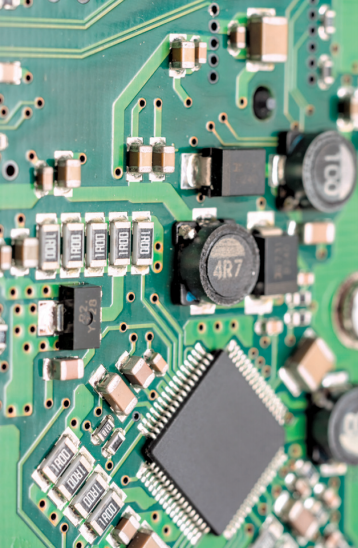
\includegraphics[scale=0.3]{figs/vlc-chips}
\end{figure}
\end{frame}
%
\begin{frame}{!分块矩阵的运算法则}
\begin{itemize}
\item 加法: 正常加, 但是要求分块类型是相同的. 
\item 数乘: 正常数乘.
\item 乘法(有意思的地方来了):
\begin{itemize}
\item 左边的列的分法要和右边的行的分法相同
\end{itemize}
\item 转置(容易错)
\begin{itemize}
\item 注意作用的``传导'', 就像链式法则一样. 
\end{itemize}
\item Def. 分块对角矩阵
\item Prop. 分块对角矩阵$|A|=|A_{1}||A_{2}|\cdots|A_{s}|$, 但是分块上三角矩阵没有这样好的性质. 
\item Prop. 分块对角矩阵的逆是每一个对角元上的逆之后的矩阵
\item Note. 分块上三角矩阵也没有这样的性质, 而是$A=\begin{pmatrix}B & D\\
 & C
\end{pmatrix},A^{-1}=\begin{pmatrix}B^{-1} & -B^{-1}DC^{-1}\\
 & C^{-1}
\end{pmatrix}.$ (很奇怪, 后面会提及)
\item Prop. 分块对角矩阵的乘积是对应相乘. 
\end{itemize}
\end{frame}
%
\begin{frame}{``复杂的东西总是存在简单的解释''}
\begin{itemize}
\item Python程序是由一条条简单的语句构成的
\item 汇编语言只有比较少(大部分)的指令
\item 我们总是用简单的东西理解世界, 并且逐步推广
\item 可逆矩阵可不可以分解为初等矩阵的乘积?
\end{itemize}
\end{frame}
%
\begin{frame}{!矩阵的初等行列变换}
\begin{itemize}
\item Def. 矩阵的初等行(列)变换
\item 可以写成矩阵相乘的形式, 赞(大大统一了形式)!
\item 考察这些``被消元之后的矩阵'', 发现了什么?
\begin{itemize}
\item 原来可是一堆方程组
\item 不妨把它们归为一类!
\end{itemize}
\item 等价类与等价关系(在相抵意义下的标准型)
\item 算法: 求线性方程组(Guass消元法, 低配版)
\begin{itemize}
\item 发现: 最后总是可以消成\textbf{阶梯型}
\begin{itemize}
\item 存在吗?唯一吗?(自行阅读证明)
\end{itemize}
\item 反应了这个线性方程组到底有几个是真正来干事的
\item Def. 秩: $A_{n\times n},r(A)=r\iff PAQ=\begin{pmatrix}I_{r} & 0\\
0 & 0
\end{pmatrix}$.
\end{itemize}
\item 联系$AX=B,XA=B$. 
\end{itemize}
\end{frame}
%
\begin{frame}{可逆矩阵可不可以分解为若干个初等矩阵的乘积?}
\begin{itemize}
\item 任意的初等行列变换都可以经过一系列初等行列变换变为标准形. 
\begin{itemize}
\item 唯一性, 存在性, 自读教科书
\end{itemize}
\item 如果$A$\textbf{可逆}, 我们只要通过初等行变换把$A$化作$I_{n}$. 假设$P_{k}...P_{1}AQ_{1}...Q_{l}=I_{n}.$
\begin{itemize}
\item (互逆的矩阵可交换) $\left(P_{k}...P_{1}A\right)Q_{1}...Q_{l}=I_{n}$.
\item $Q_{l}^{-1}P_{k}...P_{1}AQ_{1}...\mathbf{Q_{l}Q_{l}^{-1}}=Q_{l}I_{n}Q_{l}^{-1}.$
\end{itemize}
\item $A^{-1}XA$有着很好的性质, 尤其是在算幂次的时候. 
\begin{itemize}
\item 求$\left(A^{-1}XA\right)^{2},\left(A^{-1}XA\right)^{3},\cdots,\left(A^{-1}XA\right)^{n}$. 
\end{itemize}
\item 设$A=\begin{pmatrix}1 & 1\\
1 & 0
\end{pmatrix},$求$A^{2},A^{3},A^{4},A^{5}.$
\begin{itemize}
\item 要是能写成$T^{-1}\begin{pmatrix}\lambda_{1}\\
 & \lambda_{2}
\end{pmatrix}T$的样子就好了. 
\item 能不能做? 
\begin{itemize}
\item char-poly.py
\item (3阶矩阵前若干个有这些\textbf{可以}(-3..3){[}6493, 121916, \textbf{6481981}{]},(-1..1){[}747,
3882, \textbf{15054}{]},(114,514,191){[}0, 165, \textbf{19518}{]})(98\%,76\%,98\%)
\end{itemize}
\end{itemize}
\item 矩阵的\textbf{相似}
\end{itemize}
\end{frame}
%
\begin{frame}{例子: 解线性方程组}
\begin{enumerate}
\item 求方程组
\[
\begin{cases}
3x+2y+z=39 & (1)\\
2x+3y+z=34 & (2)\\
x+2y+3z=26 & (3)
\end{cases}
\]
的解.
\item 讨论线性方程组
\[
\begin{cases}
x_{1}+3x_{2}+2x_{3}=1 & (1)\\
2x_{1}+5x_{2}+\lambda x_{3}=3 & (2)\\
3x_{1}+\lambda x_{2}-8x_{3}=1 & (3)
\end{cases}
\]
的解.(Eg3.4.13)
\end{enumerate}
\end{frame}
%
\begin{frame}{跑题: Wolfram Mathematica中的Solve{[}{]}函数}
\begin{itemize}
\item Wolfram Language
\begin{itemize}
\item == 表示相等关系, =表示赋值
\item 所有的命令都是由{[}{]}
\item 完全函数式
\item 矩阵的乘法是$a.b$而不是$a*b$, $a*b$是Hadamard乘积(每一个格子对应相乘). 
\item 更多的参看Help>Wolfram Documentation
\end{itemize}
\item LinearSolve{[}{]}
\begin{itemize}
\item finds an $x$ that solves the matrix equation $m.x==b$. 
\end{itemize}
\item 例子:
\begin{itemize}
\item In{[}{*}{]}:=$\texttt{LinearSolve[\{{\{{a,b}\},\{{c,d}\}}\},\{{x,y}\}]}$
\begin{itemize}
\item 
\[
\texttt{Out[*]=}\left\{ \frac{dx-by}{ad-bc},\frac{cx-ay}{bc-ad}\right\} 
\]
\end{itemize}
\end{itemize}
\end{itemize}
\end{frame}
%
\begin{frame}{例子: 求$AX=B,XA=B$的方法}
\begin{enumerate}
\item 求$X,$使得$AX=B$, 其中$A=\begin{pmatrix}1 & 2 & 3\\
2 & 2 & 1\\
3 & 4 & 3
\end{pmatrix},B=\begin{pmatrix}2 & 5\\
3 & 1\\
4 & 3
\end{pmatrix}.$
\begin{enumerate}
\item Solution. $X=\begin{pmatrix}3 & 2\\
-2 & -3\\
1 & 3
\end{pmatrix}.$
\end{enumerate}
\end{enumerate}
\end{frame}
%
\begin{frame}{为什么翻译做秩(rank)}
\begin{itemize}
\item 《廣韻·入聲·質·秩》秩:\textbf{積}也,\textbf{次}也,\textbf{常}也,\textbf{序}也,書曰望秩于山川。直一切,十二。
\item 《孔叢子·論書》: 孔子曰:「高山『五嶽』,定其差秩,祀所視焉。」
\item 可能是暗示这是等价关系? (可能有更好的理解方式)
\end{itemize}
\end{frame}
%
\begin{frame}{!关于秩的第二个等价定义}
\begin{itemize}
\item 能不化简直接看吗? 
\begin{itemize}
\item 可以! Def. 秩(子式版本)
\begin{itemize}
\item 设$A_{m\times n}$, 则\textbf{存在}有一个$r$阶子式不为0, 且\textbf{所有}$r+1$阶子式都为0
\end{itemize}
\item 为什么要用这个? 定义多项式矩阵的秩的时候第一个就不灵了. 
\end{itemize}
\item 经过初等行(列)变换, 秩不变
\begin{itemize}
\item Def1很容易
\item Def2怎么证?
\end{itemize}
\item Def. 满秩与降秩
\begin{itemize}
\item $\begin{pmatrix}0 & 0\\
0 & 0
\end{pmatrix}$仿佛自己失了秩.jpg
\end{itemize}
\end{itemize}
\end{frame}
%
\begin{frame}{案例: 观察刚刚那个图形程序}
\begin{itemize}
\item 满秩的时候是什么情形?
\item 降秩呢?
\item 刻画了``压了多少'', 行列式没办法处理($|A|=0$)
\end{itemize}
\end{frame}
%
\begin{frame}{!问题: 矩阵相乘对于矩阵的秩有什么影响?}
\begin{itemize}
\item 观察例子!
\begin{itemize}
\item 如果乘的是个零矩阵, 就降秩了. 
\item 有没有可能升秩呢?
\item 如果两个矩阵的秩是一样的, 相乘等于什么?
\end{itemize}
\item $r(AB)\leq\min\{r(A),r(B)\}$. 
\begin{itemize}
\item 考虑标准形: $A=\begin{pmatrix}E_{r} & 0\\
0 & 0
\end{pmatrix},B=\begin{pmatrix}E_{s} & 0\\
0 & 0
\end{pmatrix}.$ $r(AB)=\min\{r(A),r(B)\}$错误的证明!
\item 小命题: $P$可逆, $r(PA)=r(A)$. (可逆矩阵是一系列初等矩阵的乘积) 根据Def1.
\item 根据定义: $PAQ=\begin{pmatrix}E_{r} & 0\\
0 & 0
\end{pmatrix},r(AB)=r(PA\mathbf{QQ^{-1}}B)=r\left(\begin{pmatrix}E_{r} & 0\\
0 & 0
\end{pmatrix}B'\right)$
\item $r(B')=r(B)$
\item $\begin{pmatrix}E_{r} & 0\\
0 & 0
\end{pmatrix}B'$是$B'$的前$r$行, 因此秩小于$r$. 
\end{itemize}
\end{itemize}
\end{frame}
%
\begin{frame}{!因此说说0}
\begin{itemize}
\item 在数的领域里面, $ab=0\implies a=0\lor b=0$
\item 矩阵里面只有$r(A)=r(B)$的时候才可以出现. 
\begin{itemize}
\item 不相等的时候无法推出$A=0\lor B=0$.
\end{itemize}
\end{itemize}
\end{frame}
%
\begin{frame}{例子: Jordan块, 伴随矩阵与秩}
\begin{enumerate}
\item 求
\[
\lim_{n\to\infty}\begin{pmatrix}1/2 & 1 & 1\\
0 & 1/3 & 1\\
0 & 0 & 1/5
\end{pmatrix}^{n}.
\]
\item 设$n$阶矩阵$A$的伴随矩阵为$A^{*}$, 证明(各个小题没有较大的关联):
\begin{enumerate}
\item $|A^{*}|=|A|^{n-1};$
\item $\left(A^{*}\right)^{*}=|A^{n-2}|A$
\item $r(A^{*})=\begin{cases}
n & r(A)=n\\
1 & r(A)=n-1\\
0 & r(A)<n-1
\end{cases}$
\end{enumerate}
\item 设$A$为$n$阶方阵, $A^{*}$为伴随矩阵, 并且$\det A=1/3$, 求$\det\left(\left(\frac{1}{4}A\right)^{-1}-15A^{*}\right)$.
\end{enumerate}
\end{frame}
%
\begin{frame}{例子: 反对称矩阵的秩}
\begin{enumerate}
\item 反对称矩阵有这样的性质: $A^{T}=-A$. 
\item 设$a,b,c$不全为0, 试着求$A=\begin{pmatrix}0 & a & b\\
-a & 0 & c\\
-b & -c & 0
\end{pmatrix}$的秩. 
\item 设$A=(a_{ij})_{n\times n}$是$n$阶反对称矩阵
\begin{enumerate}
\item 如果$n$为奇数, $|A|=0$. 
\item ({*})如果$n$为偶数, $|A|$是一个以$a_{ij}$为多项式的平方, 如果多项式的取值限制在实数范围内, 那$|A|\geq0$
\end{enumerate}
\end{enumerate}
\end{frame}
%
\begin{frame}{{*}例子(继续): 反对称矩阵的秩}
\begin{itemize}
\item 设$a,b,c$不全为0, 试着求$A=\begin{pmatrix}0 & a & b\\
-a & 0 & c\\
-b & -c & 0
\end{pmatrix}$的秩. 

一个好玩的观念如下: 
\begin{itemize}
\item 从分块矩阵的角度来看, 记录$A=\begin{pmatrix}B & \alpha\\
-\alpha & 0
\end{pmatrix},B=\begin{pmatrix}0 & a\\
-a & 0
\end{pmatrix},\alpha=\begin{pmatrix}b\\
c
\end{pmatrix}$
\item $B$可逆, 有$\begin{pmatrix}E_{2} & 0\\
\alpha^{T}B^{-1} & 1
\end{pmatrix}A\begin{pmatrix}E_{2} & -B^{-1}\\
0 & 1
\end{pmatrix}=\begin{pmatrix}B & 0\\
0 & \alpha^{T}B^{-1}\alpha
\end{pmatrix}$
\end{itemize}
\begin{enumerate}
\item 注意: 反对称矩阵的逆也是反对称的
\item 然后就说明了$(\alpha^{T}B^{-1}\alpha)=\alpha^{T}(B^{-1})^{T}\alpha=-\alpha^{T}B^{-1}\alpha$,
因此$\alpha^{T}B\alpha=0$. 
\item ({*}) 设$B_{m\times n}$是反对称矩阵, 对任意$X_{m\times1}$有$X^{T}BX=0$. 
\item ({*}) 设$B_{m\times n}$是反对称矩阵, 对任意$X_{m\times n}$有$X^{T}BX=0$. 
\begin{enumerate}
\item 矩阵的\textbf{合同}
\end{enumerate}
\end{enumerate}
\end{itemize}
\end{frame}
%
\begin{frame}{{*}例子: 初等变换解决秩的不等式(Sylvester不等式)}
\begin{enumerate}
\item 设$A_{m\times n},B_{n\times s},$那么
\[
r(AB)\geq r(A)+r(B)-n.
\]
\end{enumerate}
\end{frame}
%
\begin{frame}{{*}例子: 更多关于秩的有趣性质}
\begin{itemize}
\item $r\begin{pmatrix}A & O\\
O & B
\end{pmatrix}=r(A)+r(B)$
\item $r\begin{pmatrix}A & O\\
C & B
\end{pmatrix}\geq r(A)+r(B)$
\item $A$的子矩阵的秩$r(A_{1})\leq r(A)$.
\end{itemize}
\end{frame}
%
\begin{frame}{!回到主题: 线性方程组的求解}
\begin{enumerate}
\item 化为阶梯型: 
\[
(A|\beta)\stackrel{\text{行变换}}{\implies}\begin{pmatrix}* & * & * & *| & b_{1}\\
0 & * & * & *| & \vdots\\
0 & 0 & * & *\\
0 & 0 & 0 & *| & b_{r}\\
0 & 0 & 0 & 0| & b_{r+1}\\
0 & 0 & 0 & 0| & \vdots\\
0 & 0 & 0 & 0| & b_{n}
\end{pmatrix}
\]
\item 判断有没有解: $b_{r+1}=0,..,b_{n}=0$有解, 反之无解
\item 求$AX=\beta$的解
\begin{enumerate}
\item 考虑$AX=0$的解(有什么好处?)
\begin{enumerate}
\item $S=\{AX=0\}$的解: 加法封闭, 数乘封闭
\item 对于那些自由的变量, 取$\epsilon_{1}=(1,0,\cdots,0)^{T},\epsilon_{n}=(0,0,\cdots,1)^{T}$
\item 得到通解$X=(x_{1}..x_{n})^{T}=\sum_{i=1}^{n}x_{i}\epsilon_{i}$
\end{enumerate}
\item 考虑$AX=\beta$的解(解一一对应)
\end{enumerate}
\end{enumerate}
\end{frame}
%
\begin{frame}{Tips: 遇见线性表示的时候}
\begin{itemize}
\item 有时候记得用矩阵乘法的形式简化记号!
\[
k_{1}\eta_{1}+\cdots+k_{n}\eta_{n}=0\iff(\eta_{1}..\eta_{n})\begin{pmatrix}k_{1}\\
\vdots\\
k_{n}
\end{pmatrix}.
\]
\end{itemize}
\end{frame}
%
\begin{frame}{!可是线性方程组里有时候有废物啊!}
\begin{itemize}
\item 例子: $\begin{cases}
x+y=1 & (1)\\
2x+2y=2 & (2)
\end{cases}$
\item 什么是废物? 可以被其他人替代. 
\item 什么叫替代? 别人调整一下自己, 就能代替你的功能.
\item 嗯?
\item Def. 线性相关
\item 补充一点点命题逻辑的内容
\item Takeaway Message. 找到自己人生的道路, 别人无法替代或很难替代
\begin{itemize}
\item \href{https://www.bilibili.com/video/BV1RR4y1s73d/?spm_id_from=333.337.search-card.all.click&vd_source=92e33b8be0a9fcd124e9c9cb80f446f0}{韩老师与你“漫谈学习和人生规划”}
\item \href{https://zhuanlan.zhihu.com/p/417187798}{程序分析-第五章-聊聊太卷的学业生活}
\end{itemize}
\item 举个具体的例子:
\begin{itemize}
\item 平面坐标系:平面上任意两个不共线的向量线性无关, 任意三个向量线性相关; 
\item 空间坐标系:空间中任意三个不共面的向量线性无关, 任意四个向量线性无关.
\end{itemize}
\end{itemize}
\end{frame}
%
\begin{frame}{!极大线性无关组}
\begin{itemize}
\item Def. 极大线性无关组
\item 唯一吗?
\begin{itemize}
\item 不唯一的, 但是数量是唯一的. 
\end{itemize}
\end{itemize}
\end{frame}
%
\begin{frame}{一种特殊的分块法}
\begin{itemize}
\item 研究什么集合里面有没有废物? 向量的集合里面!
\item 允许怎样调整? \textbf{加法}和\textbf{数乘}. 
\item 其实, 这是一种特殊的分块!
\begin{itemize}
\item 行向量
\item 列向量
\end{itemize}
\item 线性方程组的向量表示
\item Def. 向量的个数和维数
\end{itemize}
\end{frame}
%
\begin{frame}{!向量的线性相关性: 进一步说明}
\begin{itemize}
\item Th1. 线性相关$\iff$至少有一个向量可由其他的向量线性表示
\item Th2. $a_{1}..a_{m}$线性无关, $a_{1}..a_{m+1}$线性相关$\implies$$a_{m+1}$可以由$a_{1}..a_{m}$唯一表示. 
\item 诶? 矩阵的行列变换的时候也有类似的``除去废物''的行为. 
\item 那么向量组的线性相关性和矩阵的秩之间有没有关系呢? 
\begin{itemize}
\item 有! Def. 行秩, 列秩. 
\end{itemize}
\end{itemize}
\end{frame}
%
\begin{frame}{!增加向量个数}
\begin{itemize}
\item Th1. 已经线性相关的向量组, 增加向量, 仍然线性相关
\item Coll1. 线性无关的向量组, 减少向量个数, 仍然线性无关
\item Th2. 已经线性无关的向量组, 增加向量组的维数, 那么仍然线性无关. 
\end{itemize}
\end{frame}

\section{{*}线性?空间?}

\begin{frame}{{*}线性空间}
\begin{itemize}
\item 总结与归纳: 线性空间的八条性质.
\item 第一个比较抽象的例子!
\item 为什么要抽象?
\begin{itemize}
\item 平面, 空间的维数还是有限的
\item 有时候维数是无限的! 
\end{itemize}
\item 多项式空间: 无穷维的, 用向量表示很多时候不灵了
\item Def. 基, 维数, 坐标
\end{itemize}
\end{frame}
%
\begin{frame}{{*}子空间}
\begin{itemize}
\item 集合的子集
\item 线性空间的子空间, Eg., Def. 子空间
\item 维数公式(和集合的很像!)
\item Def. 直和(方便很多)
\end{itemize}
\end{frame}
%
\begin{frame}{{*}线性映射}
\begin{itemize}
\item 可以不可以不去依赖基, 来阐述线性空间之间的映射呢?
\item Def. 线性变换$\varphi:V\to U$
\item 线性映射的最关键的条件是什么?
\item 我们可以做\textbf{基的转化}. Def. 过渡矩阵
\end{itemize}
\end{frame}
%
\begin{frame}{为什么要研究映射?}
\begin{itemize}
\item 转化的观点
\begin{itemize}
\item 例子: $\text{考虑}\R^{+},\text{定义}a\oplus b=ab,k\circ a=a^{k},k\in\R,a,b\in\R^{+}.\text{现在求这个空间的维数}.$
\item 不妨使用$\ln,\exp$两个在这个空间下是线性的映射来看一看, 这样我们就看到了这个空间化为了$\R$, 因此这个空间的维数就是$1$.
\end{itemize}
\end{itemize}
\end{frame}
%
\begin{frame}{线性空间的同构{*}}
\begin{itemize}
\item 对应过去的一种想法, 构造一一对应.
\item 小故事: 山头, 架桥与学习知识
\end{itemize}
\end{frame}
%
\begin{frame}{线性代数基本不讲}
\begin{itemize}
\item 为什么看上去学的没什么用? 
\begin{itemize}
\item 深度不够, 很多内容看起来不够自然
\end{itemize}
\item 缺失的不止这些!
\begin{itemize}
\item 数域, 多项式的性质...
\item (有一部分和数论很相似, 学过{[}数学/信息{]}竞赛的同学有福了)
\end{itemize}
\item 个人观点: 看一看想做什么
\begin{itemize}
\item 严肃认真的研究东西$\rightarrow$学习\textbf{高等代数}
\item \textbf{混}个毕业躺平当个码农$\rightarrow$后面的内容不用听了
\end{itemize}
\end{itemize}
\end{frame}
%
\begin{frame}{《本命年的胡思乱想》–朱富海}

想想不由得有点沮丧:尽管面对的是大学新生,每个人都是18岁上下,然而他们中的很多人似乎已经定型了。正所谓“冰冻三尺非一日之寒”,不管是求知欲的丧失、动手能力的欠缺还是逻辑思维能力的匮乏,都不是一朝一夕形成的,其根源应该在中学,或许还有小学,这大概是以后我该关注的地方。

...

跟一些中学生接触过,有的学生受到的毒害比较深,已经不会思考了;也有一些学生,尤其是低年级学生,还具有初生牛犊的锐气,他们在课余之时学了不少大学数学内容,比如,就我所知,一些中学生看过我编写的《高等代数与解析几何》和《抽象代数》,甚至看了《有限群表示论》。挺想和他们保持沟通的,可惜未能实现,他们还面临着高考的压力,我不便于过多打扰他们,他们似乎也不想打扰我。

\end{frame}

\section{{*}回顾解线性方程组的过程}
\begin{frame}{!线性方程组什么时候有解?}
\begin{itemize}
\item Th1. 有解的判定条件
\begin{itemize}
\item 无解$\iff$ $R(A)<R(A,b)$
\item 有唯一解$\iff$$R(A)=R(A,b)=n$
\item 有无穷多的解$\iff R(A)=R(A,b)<n$.
\end{itemize}
%
\end{itemize}
\end{frame}
%
\begin{frame}{!先看看右边等于0的情况}
\begin{itemize}
\item 
\[
AX=0
\]
\item Def. 基础解系
\begin{itemize}
\item 和向量的情形很相似. 
\end{itemize}
\end{itemize}
\end{frame}
%
\begin{frame}{!那么右边不等于0的时候呢}
\begin{itemize}
\item 非齐次线性方程组
\begin{itemize}
\item Prop1. 两个解相减就得到了等于0的情况
\item Prop2. 右边等于0的解系+右边等于A的解=右边等于A的解
\end{itemize}
\item 表达: 齐次的通解+特解
\item 以前的那些Ideas...
\begin{itemize}
\item 秩
\item 线性表示
\item 向量组的等价
\end{itemize}
\end{itemize}
\end{frame}
%
\begin{frame}{{*}从``0''开始: 核空间}
\begin{itemize}
\item 好像高中没有系统的讲过映射的概念
\begin{itemize}
\item 补充视频: 《离散数学》南京大学 魏恒峰 (ant-hengxin @ bilibili)
\end{itemize}
\end{itemize}
\begin{figure}
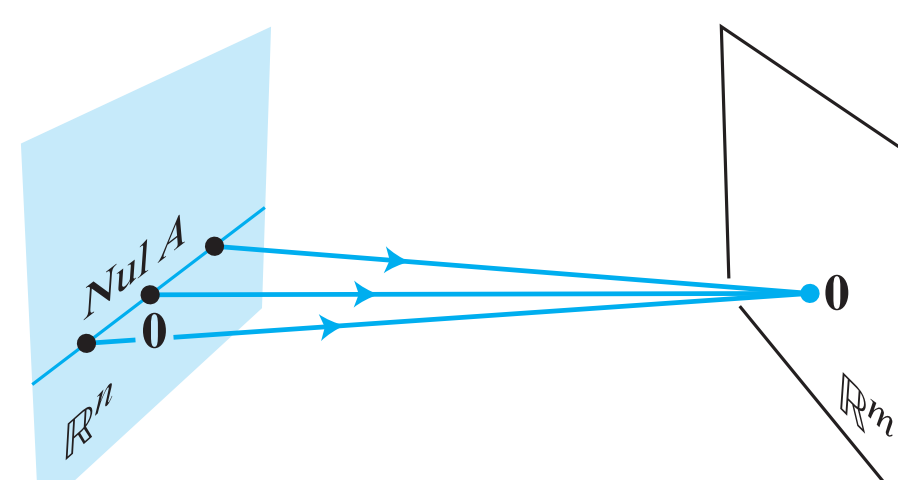
\includegraphics[width=0.8\paperwidth]{figs/ker-spaces}

\caption{核空间示意}
\end{figure}
\end{frame}
%
\begin{frame}{启示: 从基础的问题做起}
\begin{itemize}
\item 个人经历: 停课, 复课, 与课本基础题
\begin{itemize}
\item 高一: 数学课本? 那么简单的东西还要看?
\item 高二(上): 停课玩OI, 没有(学习)数学课本, 数学课程都是在网络上找的(和课外班)
\begin{itemize}
\item 啥也看不懂: 符号繁杂$\sum,\prod,d/dx,\int,\oplus,\mu,d,{n \choose m}$; 不讲人话(显然,易得,注意到...)(境界不够)
\item 没人问: 网络上, 听不懂; 现实中, 不会(学长们都忘了OI相关的数学)
\end{itemize}
\item 高二(下): 宋老师(班主任): 从基础题做起, \textbf{从课后习题}做起
\begin{itemize}
\item 但是看不到课后习题背后的内涵, 甚至没有想法去看内涵
\end{itemize}
\item 高三: 看数学课本, 小丑竟是我自己
\end{itemize}
\item Recall. 复杂的东西可以被简单的东西组合起来(不一定是线性组合)
\item 线性代数(或高等代数)的学习就多了几分\textbf{意义}
\item 不过欠下来的总是迟早要补的, 不然迟早出大麻烦(如映射, 集合, 命题逻辑). 参看《离散数学》by南京大学 魏恒峰
\begin{itemize}
\item 原因: 高考不考. 但是面对更加复杂的数学结构原来靠\textbf{直觉}有时候就不灵了. 
\end{itemize}
\end{itemize}
\end{frame}
%
\begin{frame}{《高中数学与大学数学》–朱富海}

{\footnotesize{}从学生的学习方式看, 差异很大. 很多学生都有同样的体会: 中学数学是刷题刷出来的, 或者准确地说,
中学数学给他们留下的最深(希望不是全部)的印象是刷题. 学生们总有做不完的练习题, 其中很大一部分是机械性的重复. 在大量的重复训练中,
学生们形成了条件反射, 会套用一些方法快速做题, 从而能有效应对考试. 然而这种训练方式的后果是明显的: \alert{{\footnotesize{}学生们穷于应付作业, 根本没有时间思考, 或者更严重的, 他们根本没有产生要思考的念头! }}长此以往,
他们的思维能力在退化, 接受新知识的能力也在退化, 因为没有足够的重复次数, 他们学不明白新知识. 这些都给学生的大学生活带来了隐患,
因为大学数学一般是刷题刷不出来的, 很多课程没有那么多习题供学生练习, 很多高年级的选修课的教材根本没有课后练习! 有人说数学研究不是玩技巧的,
而是玩概念的, 很有道理. 大学的很多课程都是数学家们对一些问题感兴趣, 提炼出其中共性得到一个新的概念, 围绕这个概念进行探索,
逐步建立起一个新的数学理论, 原始问题在新的理论下一步步获得解决. 这样的课程对初学者是有一定挑战性的, 光看书已经不容易懂了, 因为他们从书上看不出或者根本不关心问题的起源和探索路径,
自然也不明白为什么要讲那些看起来不那么友好的数学命题. 对大部分学生来说, 课前适当预习, 了解一下课程的框架, 带着问题听课效果会好一点,
否则课后复习难度较大. 有的学生就反映, 复习过程有时要花费比老师讲课更长的时间.}{\footnotesize\par}
\end{frame}
%
\begin{frame}{遗留的问题}
\begin{itemize}
\item 基1 $\rightarrow$ 线性映射 $\rightarrow$ 基2
\item 有时候基麻烦了, 怎么换?
\item 我们还能用矩阵表示什么?
\end{itemize}
\end{frame}
%
\begin{frame}{参考视频、文章与书籍}
\begin{itemize}
\item 《工程高等代数》中国地质大学出版
\item 《高等代数与解析几何》 朱福海等
\item 《线性代数学习指导》 李尚志
\item 《高等代数教学笔记》微信公众号, 数林广记, 朱福海
\item 《教学感悟》 微信公众号, 数林广记, 朱福海
\item 《南京大学 高等代数》bilibili zhufuhainj
\end{itemize}
\end{frame}

\end{document}
